\part{Progettazione di un'interfaccia grafica per la compressione di immagini}

L'interfaccia grafica è realizzata con l'ambiente di sviluppo QT\cite{qt}, il quale permette di creare delle GUI scrivendo il codice in linguaggio c++. La compressione applicata è stata limitata solamente alla visualizzazione, ovvero l'immagine perde l'informazione legata alle alte frequenze, però le strutture dati che contengono tale immagine rimangono costanti. Introducendo però la possibilità ad un successivo salvataggio dell'immagine, nel quale si possono memorizzare solamente i coefficienti diversi da 0.

Il programma fornisce una schermata nella quale è possibile selezionare l'immagine da comprimere e i valori di compressione da applicare. Nella sezione di sinistra viene mostrata l'immagine originale, mentre in quella di destra la sua versione compressa. In figura\ref{fig:deer} è riportato un esempio sull'immagine \textit{deer}, sulla quale sono stati applicati blocchi di elevate dimensioni (70x70) ed una elevata compressione (circa del 92\%), in questo modo è facilmente osservabile l'effetto che si ottiene sull'immagine.

Una feature fondamentale per la rapida compressione dell'immagine è stata l'aggiunta dei thread, in questo modo, suddividendo il lavoro, la compressione diventa quasi istantanea. Tale aggiunta è applicabile per via dell'indipendenza dei blocchi tra loro, infatti è possibile allocare la memoria, eseguire la compressione su tale porzione di dati e scrivere i pixel nell'immagine, senza la necessità di interagire con gli altri blocchi.

\begin{figure}[h]
	\centering
	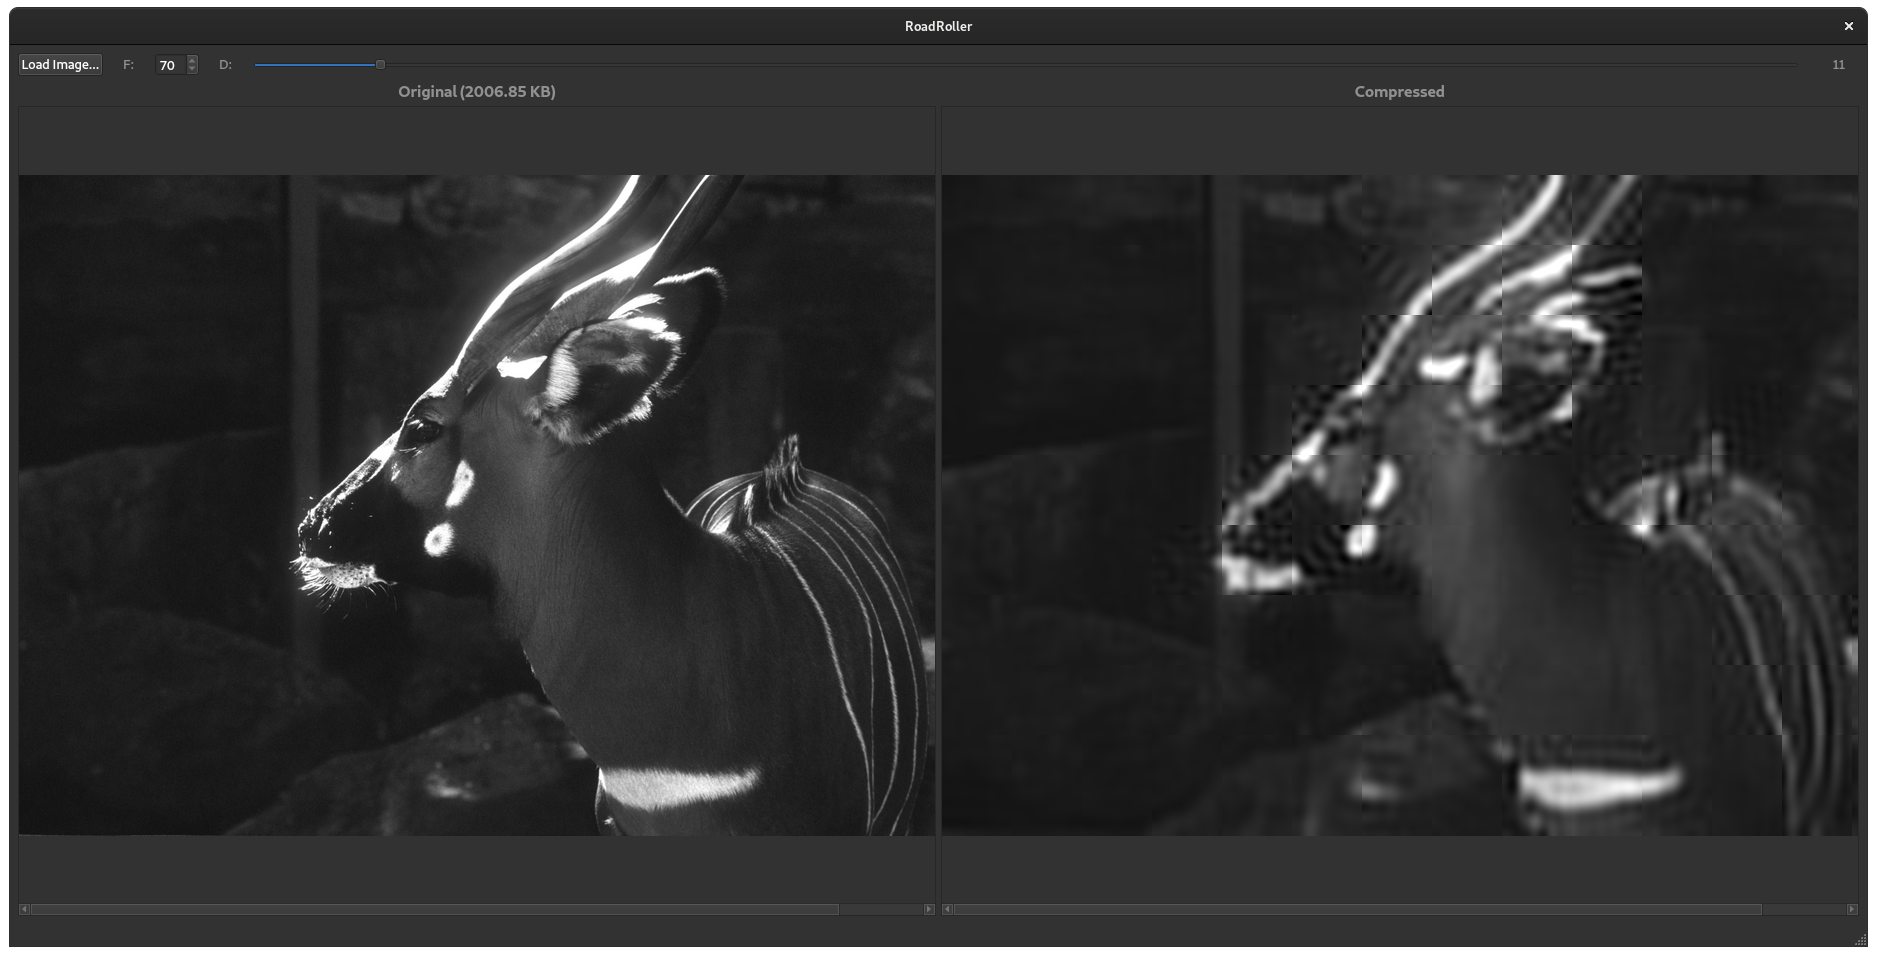
\includegraphics[width=1\linewidth]{figures/qt_deer}
	\caption{Programma di compressione con Qt}
	\label{fig:deer}
\end{figure}


Per mostrare meglio la compressione potremmo momentaneamente ignorare la conversione dei valori tramite la IDCT2. In figura\ref{fig:compression_values} viene mostrato il risultato ottenuto, dove è possibile osservare i coefficienti generati dalla DCT, i quali vengono successivamente tagliati per il valore di input scelto. In questo modo ogni blocco conterrà dati diversi da 0 solamente nella parte superiore del taglio.

\begin{figure}[h]
	\centering
	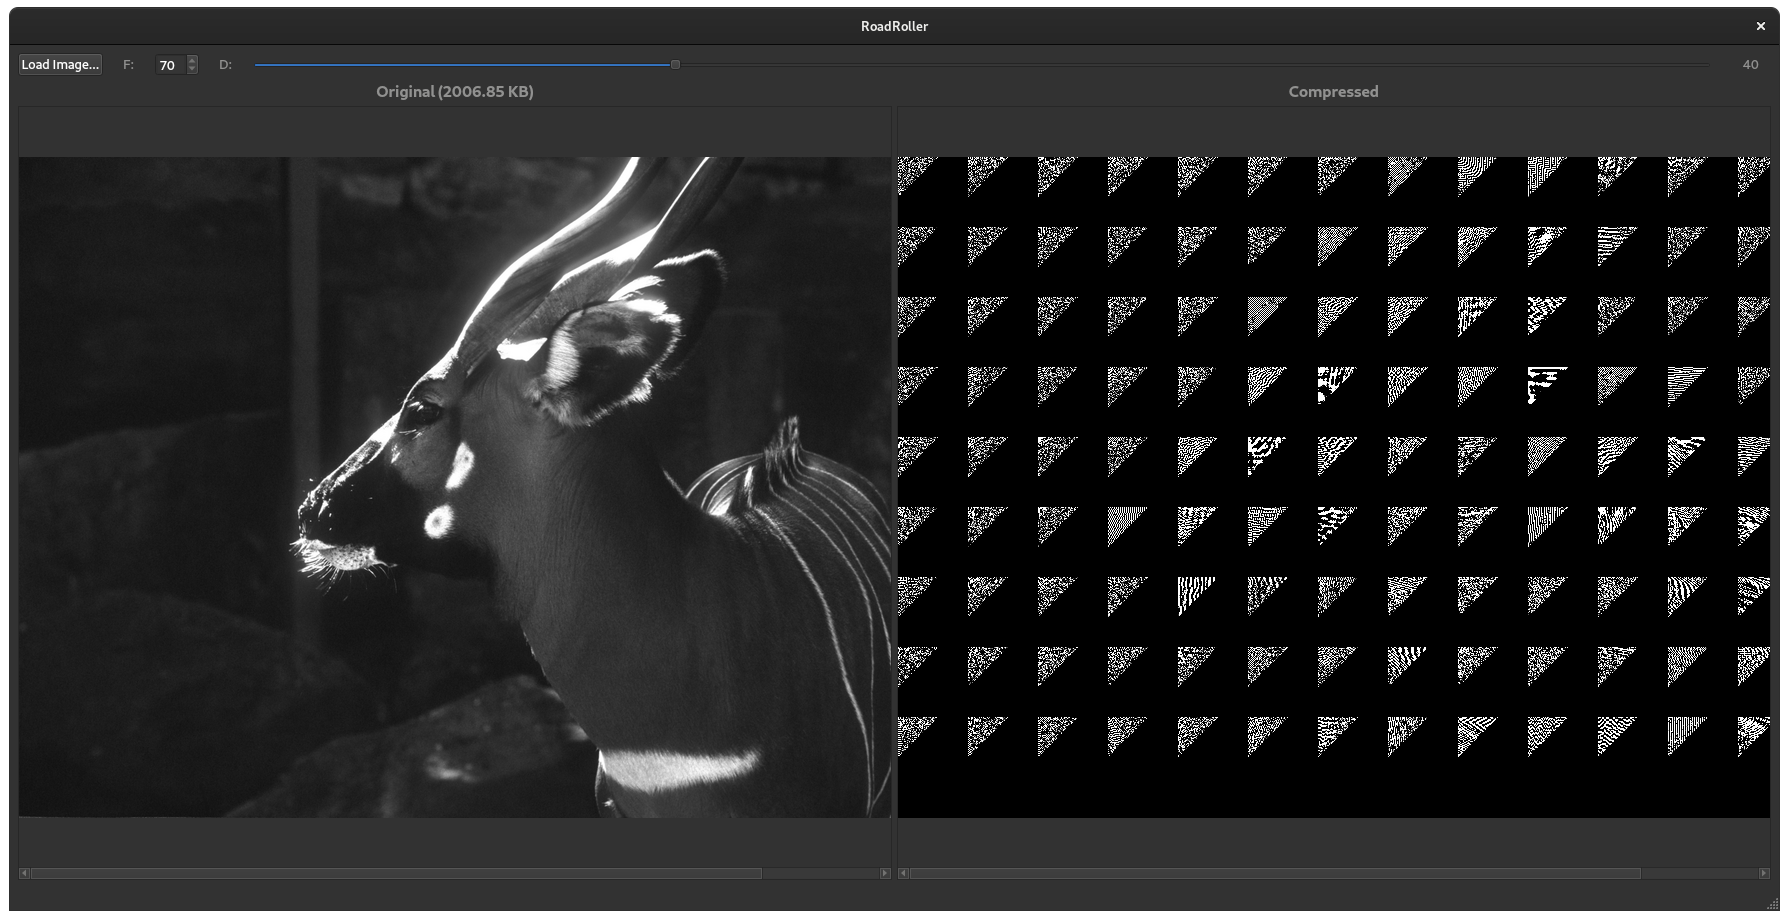
\includegraphics[width=1\linewidth]{figures/qt_dct_values}
	\caption{Valori della DCT generati dalla compressione}
	\label{fig:compression_values}
\end{figure}
